% Chapter 4

\chapter{Analysis and Design} % Main chapter title
\label{chap:Chapter4}

This chapter starts by presenting the Requirements Engineering which consists in the design of software requirements, in the form of functional and non-functional requirements.
After that, is described the logic view, the process view and the design of the functional requirements
Lastly is presents the deployment view.

\section{Requirements Engineering}

This section presents the process of analyzing the functional and non-functional requirements of this project.
The FURPS\cite{eeles2005capturing} is a system to classify requirements and represented them by categories.
It is also an acronym that represents:

\begin{itemize}
    \item \textbf{Functionality} is concerned with characteristics such as the main project features.
    \item \textbf{Usability} is concerned with characteristics such as aesthetics and consistency in the user interface.
    \item \textbf{Reliability} is concerned with characteristics such as availability, accuracy of system calculations and the system's ability to recover from failure.
    \item \textbf{Performance} is concerned with characteristics such as throughput, response time, recovery time, start-up time and shutdown time.
    \item \textbf{Supportability} is concerned with characteristics such as testability, adaptability, maintainability, compatibility, configurability, installability, scalability and localizability.
\end{itemize}

This was the system used to present and classify these categories in regards to this project.

\subsection{Functional Requirements}

This section will contain information regarding the functional requirements of the system, in the form of use cases.
These requirements generally represent the main product features and are presented in the Figure~\ref{fig:ucDiagram}.

\begin{figure}[H]
\centering
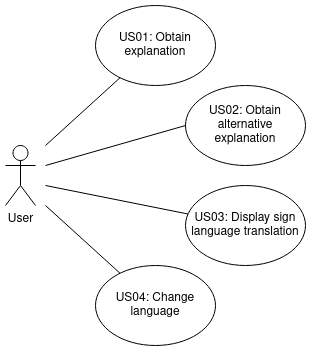
\includegraphics[scale=0.65]{ch4/assets/usecasediagram.png}
\caption[Use Case Diagram]{Use Case Diagram}
\label{fig:ucDiagram}
\end{figure}

\subsubsection{US01: Obtain explanation}

The user requests the system to present the explanation of a given word or expression.
The system generates explanations and presents, the first in the list, to the user.

\subsubsection{US02: Obtain alternative explanation}

After US01 happens.
The user gives negative feedback to the generated explanation.
The system presents the option to generate a new one.
The user selects the option for a new explanation.
The system selects the next explanation on the list or generates a new one if there are none.

\subsubsection{US03: Display sign language translation}

After the US01 happens.
The user requests the translation of the explanation to sign language.
The system sends the explanation text to the avatar API.
The API returns the animation required to perform the translation.
The integrated avatar performs the animations.

\subsubsection{US04: Change language}

The user requests the system to change the system language.
The system provides the available languages.
The user selects the desired language.
The system updates and saves the information.

\subsection{Non-functional Requirements}

The remaining "URPS" categories describe non-functional requirements that are architecturally significant.

\subsubsection{Usability}

\begin{itemize}
    \item \textbf{User Interaction} - The interaction with the user must be simple and very intuitive, taking in consideration the target audience special needs.
    \item \textbf{Help} - The system must provide suitable and contextualized help to the task the user is performing.
    \item \textbf{Interface} - It is required that the interface has to be appealing and easy to read, once again, taking in consideration the target audience special needs.
    \item \textbf{Error Prevention} - The system must prevent user mistakes and treat them accordingly.
\end{itemize}

\subsubsection{Reliability}

\begin{itemize}
    \item \textbf{Availability} - The system should have a very high availability rate.
    \item \textbf{Predictability} - The system should be reliable, that is, free of technical errors.
    \item \textbf{Fault Tolerance} - The system should be error-tolerant to protect the user from unintentional errors.
\end{itemize}

\subsubsection{Performance}

\begin{itemize}
    \item \textbf{Response Time} - The system's response time should be fast to provide quick access to data.
\end{itemize}

\subsubsection{Supportability}

\begin{itemize}
    \item \textbf{Testability} - The system should be easily testable in order to provide high confidence about correctness.
    \item \textbf{Maintainability} - The system should have high maintainability, in order to allow future requirements and/or repairs.
    \item \textbf{Configurability} - The system should support easy configurability, in order to allow adding new features.
    \item \textbf{Localizability} - The system should support multiple languages.
\end{itemize}

\section{Logic View}

A logic view represents the principal components of the application, and their interactions, that will compose the system.
The architecture proposed to be implemented is shown in Figure~\ref{fig:cd}.

\begin{figure}[H]
\centering
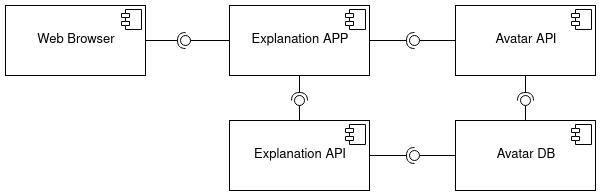
\includegraphics[width=\textwidth,keepaspectratio]{ch4/assets/component_diagram.png}
\caption[Component Diagram]{Component Diagram}
\label{fig:cd}
\end{figure}

The components presented in the above image are the following:

\begin{itemize}
    \item \textbf{Explanation App} - This component is responsible for processing the users input and converting the APIs output to the Web Browser.
    \item \textbf{Explanation API} - This component is responsible for generating an explanation for a given string.
\end{itemize}

The components already developed that will be integrated are the following:
\begin{itemize}
    \item \textbf{Avatar API} - This component is responsible for converting a given string to sign language.
    \item \textbf{Avatar DB} - This component is responsible for storing all the animations required to translate a language to their respective sign language (e.g. Portuguese to \gls{LGP}).
\end{itemize}

\subsection{Design alternative}

The main goal was initially the development of a web application that was capable of showing the users an explanation of a word or expression.
Like so the application was envisioned to take the input generate the explanation and show it to the user, like its shown in Figure~\ref{fig:ocd}.

\begin{figure}[H]
\centering
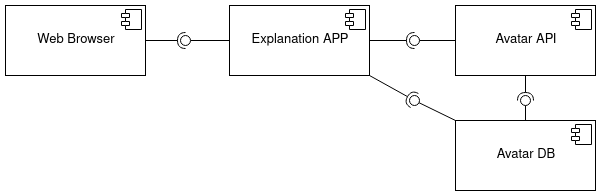
\includegraphics[width=\textwidth,keepaspectratio]{ch4/assets/component_diagram_alternative.png}
\caption[Alternative Component Diagram]{Alternative Component Diagram}
\label{fig:ocd}
\end{figure}

The disadvantage of this design in comparison with the one previously presented is that, in this one, the back end of the web application would produce the explanation.
This wouldn't allow to easily reutilize the main functionality of the application which is the generation of an explanation.
In GILT there are projects that would benefit from this feature and therefore the design had to be changed.

\section{Process View}

The first step to design a possible solution was to create a high-level view of the main functionalities the application should have.
In the flowchart of Figure~\ref{fig:Diagram1} is shown the main build blocks of the application to be developed.

\begin{figure}[H]
\centering
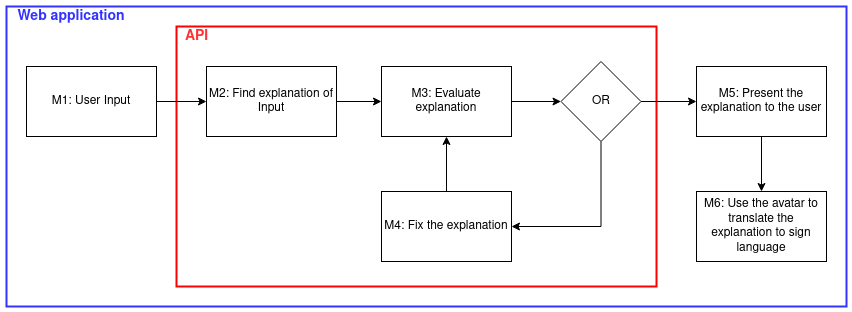
\includegraphics[width=\textwidth,keepaspectratio]{ch4/assets/diagram1_2.png}
\caption[Application Flowchart]{Application Flowchart}
\label{fig:Diagram1}
\end{figure}

The input received in M1 is send to the \gls{API} that generates an explanation in M2, which is validated in M3.
From there the explanation might be sent back to the application and shown to the user in M5  or if does not meet all the criteria defined in M3 it will be fixed in M4 and reevaluated.
After presenting the explanation to the user, the application will also be capable of sending the text to an already existing \gls{API} that is capable of translate plain text to sign language using a avatar in M6.

To help better understand the created design, a more detailed view, is presented below using activity diagrams, that describe each of the build blocks and how will they achieve the tasks previously mentioned.
The activity diagram shows the flow of a functionality, the activities that compose that functionality and the decision making required and its consequences.

The activity diagram of Figure~\ref{fig:M1}, shows the M1 block that was designed to receive a input string from the user.

\begin{figure}[H]
\centering
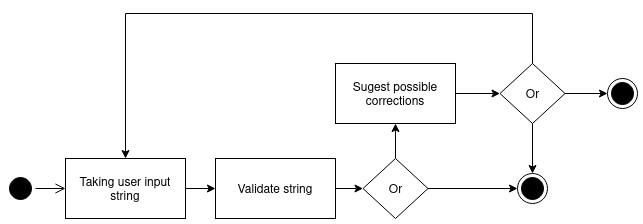
\includegraphics[width=\textwidth,keepaspectratio]{ch4/assets/M1.png}
\caption[Activity Diagram User Input Module]{Activity Diagram - M1 User Input}
\label{fig:M1}
\end{figure}

This string is validated in order to detect common mistakes, such as typos, and when an mistake is detected the application suggests possible corrections.
The user is then capable of accepting the suggestion given, make a manual correction or proceed without changing the input string.

The Figure~\ref{fig:M2} activity diagram of the M2 block, shows the process of finding an explanation based on the received string.

\begin{figure}[H]
\centering
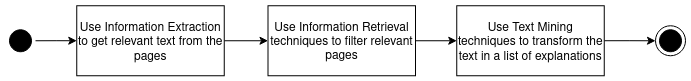
\includegraphics[width=\textwidth,keepaspectratio]{ch4/assets/M2.png}
\caption[Activity Diagram Find Explanation Module]{Activity Diagram - M2 Find Explanation}
\label{fig:M2}
\end{figure}

Information Retrieval techniques would be use to find all the pages connected to a predefined starting page, such as Wikipedia or a dictionary.
From this point, it would filter the pages that may contain information that is related to the received string.
The filtered pages would then be processed using Information Extraction techniques in order to filter the text that has some degree of relation with the initial string.
An explanation will the be generated by implementing Text Mining techniques to the blocks of text obtained from the previous step.

In Figure~\ref{fig:M3}, the activity diagram of the M3 block presents the evaluation criteria defined in order to defined an explanation as valid in order to be presented to the user.

\begin{figure}[H]
\centering
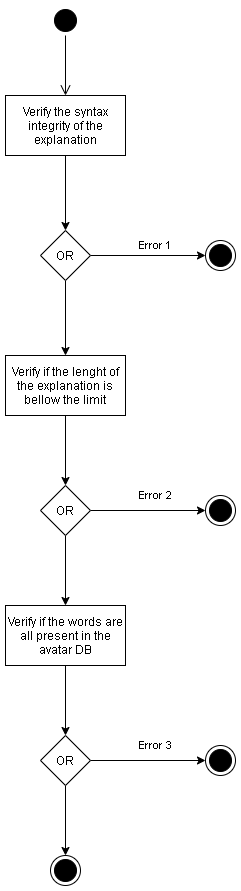
\includegraphics[width=\textwidth,keepaspectratio]{ch4/assets/M3.png}
\caption[Activity Diagram Evaluate Explanation Module]{Activity Diagram - M3 Evaluate Explanation}
\label{fig:M3}
\end{figure}

The criteria presented in the above image are the following:

\begin{itemize}
    \item \textbf{Syntax integrity} - The explanation follows syntax rules, or in other words, is a coherent sentence that can be understand when read.
    \item \textbf{Word count limit} - The explanation string needs to be shorter than a predefined value.
    \item \textbf{Compatibility with the avatar \gls{DB}} - The explanation string, ideally, needs to be composed only by words already exiting in the avatar \gls{DB}.
\end{itemize}

If a criterion fails, the error is set, and the process progresses with M4.
If a received explanation meets all the criteria it will be sent back to the web application, and the process progresses with M5.

As it can be seen in the activity diagram of Figure~\ref{fig:M4}, the M4 block is responsible for restructuring the explanation in order to meet the previously mention criteria.

\begin{figure}[H]
\centering
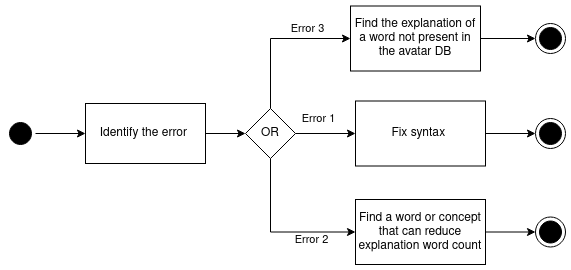
\includegraphics[width=\textwidth,keepaspectratio]{ch4/assets/M4.png}
\caption[Actibity Diagram Fix Explanation Module]{Activity Diagram - M4 Fix Explanation}
\label{fig:M4}
\end{figure}

This starts by identifying the error that made the explanation not be valid to progress and take action accordingly.

\begin{itemize}
    \item In order to fix a faulty syntax integrity, the string needs to be processed and restructured following syntax rules.
    \item In order to fix a string above a word count limit, the string needs to be analyzed to, ideally, find a word or concept that can replace a portion of the string.
    \item In order to fix incompatibilities with the avatar \gls{DB}, the words that need to be replaced, an explanation might be generated and be presented as an hypermedia link to the missing word.
\end{itemize}

The new string will then be reevaluated by the M3 block.

In the Figure~\ref{fig:M5} activity diagram, the M5 block will be displaying the generated explanation as text and hyperlinks to pages, related with the input string, to the user.

\begin{figure}[H]
\centering
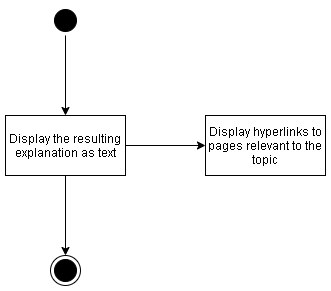
\includegraphics[width=\textwidth,keepaspectratio]{ch4/assets/M5.png}
\caption[Activity Diagram Present Explanation Module]{Activity Diagram - M5 Present Explanation}
\label{fig:M5}
\end{figure}

In this block, if the explanation had compatibility issues in M3, then those faulty words will be also be presented as hypermedia with an explanation of them.

Shown in the activity diagram of Figure~\ref{fig:M6}, is the M6 block that will take the explanation text and send it to the avatar \gls{API}.

\begin{figure}[H]
\centering
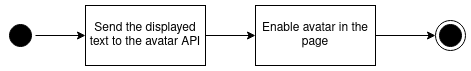
\includegraphics[width=\textwidth,keepaspectratio]{ch4/assets/M6.png}
\caption[Activity Diagram Avatar Module]{Activity Diagram - M6 Avatar}
\label{fig:M6}
\end{figure}

The avatar will appear in the web page, and will translate the received text to sign language.

With the complete design of the application in mind a simpler and easier to implement approach was design, also known as a \gls{MVP}.
This is presented in the Figure~\ref{fig:mvp}.

\begin{figure}[H]
\centering
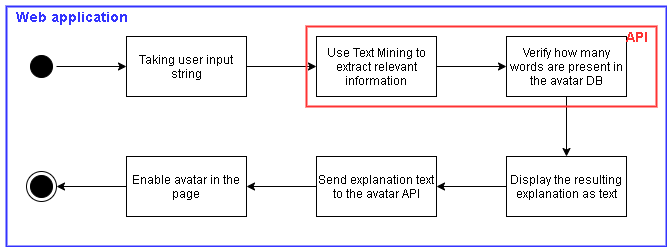
\includegraphics[width=\textwidth,keepaspectratio]{ch4/assets/mvp_2.png}
\caption[Flowchart Minimun Value Product]{Flowchart - Minimum Value Product}
\label{fig:mvp}
\end{figure}

The activity diagram shown in the above image, shows the starting point of the solution to be developed.
As a \gls{MVP}, this design focus on the key functionalities that the solution must have, removing everything else.
The major benefit of choosing this approach is allowing a fast developed of a prototype that can be used to receive feedback from the target audience, in order to grantee that the solution is going towards their needs.

\section{Functional Requirements Design}

This section is dedicated to presenting the sequence diagrams of the created use cases that were briefly explained in the Requirements Engineering section.
A sequence diagram is used to describe the objects involved in a functionality and their interactions arranged in a time sequence.

\subsection{US01: Find Explanation}

Displayed in the sequence diagram of Figure~\ref{fig:sdus01} is the design for finding an explanation.

\begin{figure}[H]
\centering
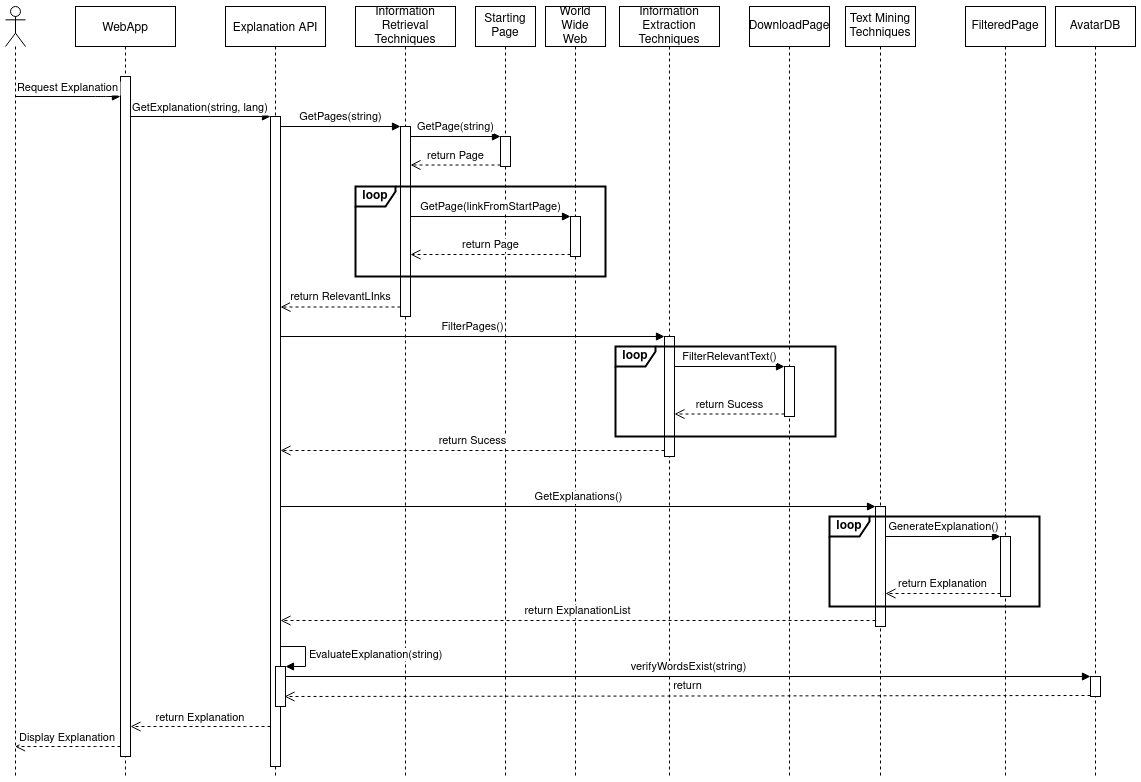
\includegraphics[width=\textwidth,keepaspectratio]{ch4/assets/US01_SD.png}
\caption[Sequence Diagram US01]{Sequence Diagram - US01}
\label{fig:sdus01}
\end{figure}

The users starts by requesting an explanation for a word/expression.
This makes the Web Application request an explanation to the Explanation API, sending the text string and the web application language (e.g. Portuguese, English, etc.).
To generate an explanation, the Explanation API passes the received string to the Information Retrieval system.
The Information Retrieval system requests and stores the starting page related to the string (e.g. for the word "king", getting the wikipedia page for king).
After the initial page, it requests and stores all the pages from the hyperlinks presented in the initial page and returns its links.
Once all the pages are gathered, the Explanation API requests the Information Extraction system to filter all the obtained pages.
To accomplish this, the Information Extraction system filters the useful text from the surrounding noise (e.g. HTML tags) and stores it in new pages.
Having now pages with only natural language, the Explanation API requests the Text Mining system to generate explanations from all filtered pages.
In order to perform this task, the Text Mining system applies text mining techniques to convert the text in each page to an explanation and return a list of explanations in the end.
With a list of explanations, the Explanation API takes the first of the list, evaluates it and returns it to the Web Application.
To conclude, the Web Application displays the explanation to the user.

\subsection{US02: Obtain alternative explanation}

Shown in Figure~\ref{fig:sdus02} is the sequence diagram that describes how the system obtains an alternative explanation.

\begin{figure}[H]
\centering
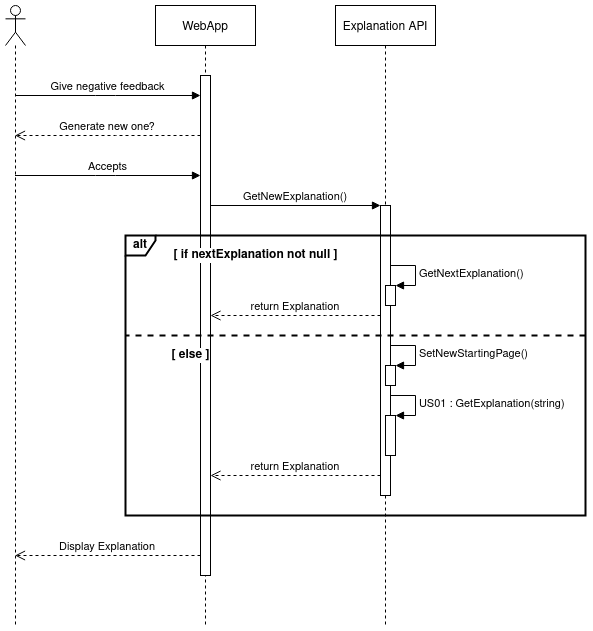
\includegraphics[scale=0.45]{ch4/assets/US02_SD.png}
\caption[Sequence Diagram US02]{Sequence Diagram - US02}
\label{fig:sdus02}
\end{figure}

The user starts by giving negative feedback to a displayed explanation.
This makes the Web Application ask if the user wants a new explanation.
The user proceeds to accept it.
Then, the Web Application requests a new explanation to the Explanation API.
If the API has more explanation in the list of generated explanation, it returns the next on the list.
Otherwise, the API sets a new starting page from a list of predefined starting pages and initiates a process of generating explanations like presented in US01.
After generating the new list of explanation it returns the first explanation to the Web Application.
To conclude, the Web Application displays the new explanation.

\subsection{US03: Display sign language translation}

In Figure~\ref{fig:sdus03} sequence diagram is shown how a translation to sign language occurs.

\begin{figure}[H]
\centering
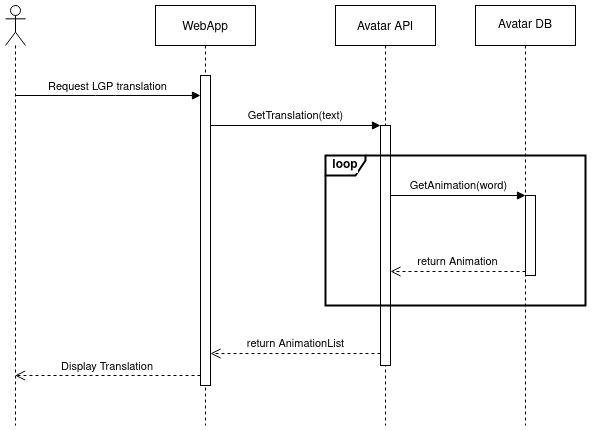
\includegraphics[scale=0.45]{ch4/assets/US03_SD.png}
\caption[Sequence Diagram US03]{Sequence Diagram - US03}
\label{fig:sdus03}
\end{figure}

The user starts by requesting the translation of a displayed explanation.
This makes the Web Application request the translation of the text to the Avatar API, sending the text and the web application language (e.g. Portuguese, English, etc.).
To accomplish this, the Avatar API queries the Avatar DB for the animations required to translate each word to the respective sign language.
The Avatar API then returns the list of the animation required to be performed in order to display the translation.
To conclude, the Web Application displays the translation using the animations in the obtained list.

\subsection{US04: Change language}

The sequence diagram displayed in Figure~\ref{fig:sdus04} presents how a change in the application language occurs.

\begin{figure}[H]
\centering
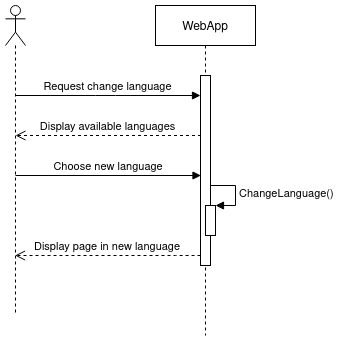
\includegraphics[scale=0.45]{ch4/assets/US04_SD.png}
\caption[Sequence Diagram US04]{Sequence Diagram - US04}
\label{fig:sdus04}
\end{figure}

The user starts by requesting the Web Application to change the language.
This makes the Web Application show a list of available language which were previously defined.
In order for a language to be eligible to appear in this list, the Avatar and the Text Mining technology needs to support it.
The user then proceeds to select one of the available languages.
To conclude, the Web Application saves the change and updates the page to the selected language.

\section{Deployment View}

A deployment view is used to view and describe the topology of the physical components of a system.
This view takes in consideration some of the non-functional requirements of the system such as, performance, scalability, availability and reliability.
The Figure~\ref{fig:deploy} presents the deployment diagram created for this project.

\begin{figure}[H]
\centering
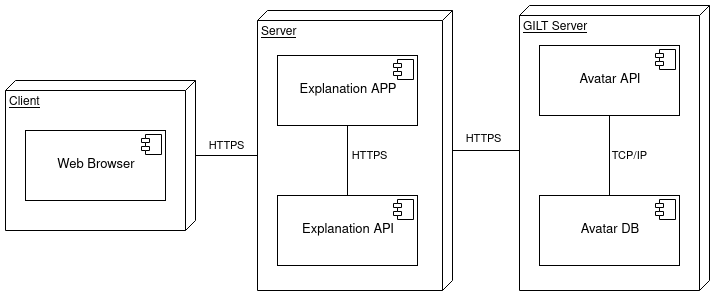
\includegraphics[width=\textwidth,keepaspectratio]{ch4/assets/deployment_diagram.png}
\caption[Deployment Diagram]{Deployment Diagram}
\label{fig:deploy}
\end{figure}

As shown in the above image, the two components to be developed, namely Explanation App and Explanation API will be hosted in the same server.
The server provider is not yet defined, but initially should be the DEI-ISEP, which is the ISEP computer engineering department.
In regards to the avatar technology, it is already hosted in a server form GILT.
Lastly, the Web Browser component will be in the client device.
